\documentclass[11pt,a4paper]{article}

\usepackage[margin=1in]{geometry}
\usepackage[T1]{fontenc}
\usepackage{lmodern}
\usepackage{microtype}
\usepackage{amsmath,amssymb}
\usepackage{booktabs}
\usepackage{array}
\usepackage{graphicx}
\usepackage{xcolor}
\usepackage{hyperref}
\usepackage{listings}
\usepackage{tikz}
\usetikzlibrary{arrows.meta,positioning,shapes.geometric}

\hypersetup{
  colorlinks=true,
  linkcolor=blue!50!black,
  citecolor=blue!50!black,
  urlcolor=blue!50!black,
  pdftitle={PulseLex: A Morse-Inspired Error-Correcting Alphabet},
  pdfauthor={PulseLex Research Prototype}
}

\title{\textbf{PulseLex: A Morse-Inspired Fixed-Length Alphabet\\
with Single-Bit Error Correction}}
\author{Independent Research Prototype}
\date{Version 0.1.0 \quad \today}

\begin{document}
\maketitle

\begin{abstract}
This paper introduces PulseLex, an experimental text-encoding design inspired
by the dot-and-dash representation of International Morse code. Instead of
using variable-length Morse symbols, PulseLex maps each supported character
to a five-bit payload, renders binary zero and one as dot and dash pulses, and
adds four parity bits using a Hamming-style $(9,5)$ block code. The resulting
code is designed to correct any single-bit error within a nine-pulse block,
provided block synchronization is known. We define the symbol alphabet,
derive the parity equations, describe a reproducible binary symmetric channel
experiment, and identify the trade-off between reliability and transmission
length. The project is an educational prototype and does not claim novelty
for Morse or Hamming coding themselves.
\end{abstract}

\section{Introduction}
International Morse code represents letters and other characters through
sequences of dots and dashes. Its international form is specified in
ITU-R Recommendation M.1677-1 \cite{itu2009morse}. PulseLex asks a different
engineering question: can a fixed-size pulse alphabet make character
segmentation straightforward while adding a small amount of error correction?

The motivation is not to replace Morse. Morse is a mature signaling system
with timing conventions and operational history. PulseLex is a controlled
experiment in combining a simple visual pulse alphabet with block coding.

\section{Research Question and Hypotheses}
The main research question is:

\begin{quote}
Can a fixed-length, Hamming-coded Morse-inspired alphabet reduce symbol
errors over an independent bit-flip channel compared with uncoded fixed-width
symbols, and what transmission-length cost does this introduce?
\end{quote}

We test three hypotheses:
\begin{enumerate}
  \item For low bit-error probabilities, Hamming-coded symbols have a lower
  symbol error rate than uncoded five-bit symbols.
  \item The code increases pulse slots per symbol from five to nine, an
  80\% increase before framing overhead.
  \item At sufficiently high error rates, multiple errors within a block
  exceed the guaranteed correction capability.
\end{enumerate}

\section{Symbol Alphabet}
Five payload bits provide $2^5=32$ possible values. PulseLex assigns values
as shown in Table~\ref{tab:alphabet}.

\begin{table}[h]
\centering
\caption{PulseLex payload allocation.}
\label{tab:alphabet}
\begin{tabular}{cl}
\toprule
Value range & Meaning \\
\midrule
0--25 & A--Z \\
26 & Space \\
27 & Period \\
28 & Comma \\
29 & Question mark \\
30 & Start marker \\
31 & End marker \\
\bottomrule
\end{tabular}
\end{table}

A payload bit of zero is displayed as a dot (\texttt{.}); a payload bit of one
is displayed as a dash (\texttt{-}). The mapping is deliberately simple and
does not reproduce the historical Morse assignment.

\section{Code Construction}
We use a systematic Hamming-style $(9,5)$ code. The five data bits
$d_1,\ldots,d_5$ occupy one-indexed positions 3, 5, 6, 7, and 9. Parity bits
occupy positions 1, 2, 4, and 8. Even parity gives

\begin{align}
p_1 &= d_1 \oplus d_2 \oplus d_4 \oplus d_5,\\
p_2 &= d_1 \oplus d_3 \oplus d_4,\\
p_4 &= d_2 \oplus d_3 \oplus d_4,\\
p_8 &= d_5.
\end{align}

The transmitted codeword is
\[
  c=(p_1,p_2,d_1,p_4,d_2,d_3,d_4,p_8,d_5).
\]
The parity-check columns correspond to the nonzero four-bit binary
representations of positions 1 through 9. Therefore a single flipped bit
produces a nonzero syndrome identifying its position. This is the standard
single-error-correction principle associated with Hamming codes
\cite{hamming1950}.

\subsection{Worked example}
For the letter A, the payload value is zero, so all five data bits are zero.
All parity bits are also zero, giving the codeword
\[
  000000000 \quad \longrightarrow \quad \texttt{.........}.
\]
If the sixth bit flips, the received block is
\[
  000001000.
\]
The syndrome identifies position six, allowing the decoder to flip that bit
back and recover A.

\section{Encoding and Decoding Workflow}
Figure~\ref{fig:workflow} summarizes the protocol.

\begin{figure}[h]
\centering
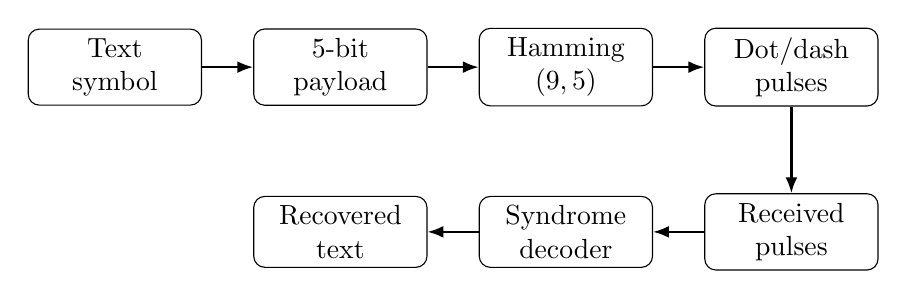
\begin{tikzpicture}[
  node distance=0.75cm and 0.65cm,
  block/.style={draw,rounded corners,align=center,minimum width=2.2cm,minimum height=0.85cm},
  arrow/.style={-{Latex[length=2mm]},thick}
]
\node[block] (text) {Text\\symbol};
\node[block,right=of text] (payload) {5-bit\\payload};
\node[block,right=of payload] (hamming) {Hamming\\$(9,5)$};
\node[block,right=of hamming] (pulse) {Dot/dash\\pulses};
\node[block,below=1.1cm of pulse] (receive) {Received\\pulses};
\node[block,left=of receive] (decode) {Syndrome\\decoder};
\node[block,left=of decode] (recover) {Recovered\\text};
\draw[arrow] (text) -- (payload);
\draw[arrow] (payload) -- (hamming);
\draw[arrow] (hamming) -- (pulse);
\draw[arrow] (pulse) -- (receive);
\draw[arrow] (receive) -- (decode);
\draw[arrow] (decode) -- (recover);
\end{tikzpicture}
\caption{PulseLex encoding and decoding path.}
\label{fig:workflow}
\end{figure}

Each character occupies exactly nine pulse units. Blocks are separated in
the text representation by whitespace. A physical implementation would need
a synchronization strategy; the present prototype assumes the receiver
already knows the block boundaries.

\section{Mathematical Analysis}

\subsection{Code rate and redundancy}
The code rate is
\[
  R=\frac{k}{n}=\frac{5}{9}\approx 0.556.
\]
Four of the nine transmitted bits are redundant. Relative to the five-bit
payload, the redundancy overhead is
\[
  \frac{9-5}{5}\times 100\%=80\%.
\]
Thus PulseLex spends 80\% more pulse slots per symbol than the uncoded
five-bit representation.

\subsection{Uncoded symbol error probability}
Assume each bit independently flips with probability $p$. An uncoded
five-bit symbol is correct only if all five bits remain unchanged:
\[
  P_{\mathrm{uncoded,error}}=1-(1-p)^5.
\]
For $p=0.01$, this is approximately $0.04901$.

\subsection{Guaranteed correction region}
The minimum Hamming distance is $d_{\min}=3$. A code with minimum distance
$d_{\min}$ can guarantee correction of
\[
  t=\left\lfloor\frac{d_{\min}-1}{2}\right\rfloor
\]
errors. PulseLex therefore guarantees correction of one bit error per block.
The probability of two or more flips in a nine-bit block is
\[
 P_{\geq 2}=1-(1-p)^9-9p(1-p)^8.
\]
At $p=0.01$, this probability is approximately $0.00343$. This is the
probability of leaving the guaranteed correction region, not necessarily the
exact decoded symbol-error probability: some multi-error patterns may decode
to the original payload, while others may be miscorrected.

\section{Experimental Method}
The implementation includes a seeded Monte Carlo simulator. For each
bit-error probability, it:
\begin{enumerate}
  \item samples a uniformly random five-bit symbol;
  \item transmits the raw payload through an independent bit-flip channel;
  \item encodes the same payload using the $(9,5)$ code and transmits it;
  \item decodes both streams and records symbol errors;
  \item repeats the process for a fixed number of trials.
\end{enumerate}

The experiment uses a binary symmetric channel. It does not model burst
errors, pulse-duration distortion, timing drift, synchronization loss, or
radio propagation. The random seed and trial count are recorded to support
reproducibility.

\section{Results}
Table~\ref{tab:results} reports the seeded reference run with 50,000 trials
at each channel probability. The complete data are included in
\texttt{results/bit\_error\_experiment.csv}.

\begin{table}[h]
\centering
\caption{Monte Carlo symbol error rates (50,000 trials per row, seed 7).}
\label{tab:results}
\begin{tabular}{ccc}
\toprule
Bit error probability $p$ & Uncoded 5-bit SER & PulseLex $(9,5)$ SER \\
\midrule
0.001 & 0.004740 & 0.000000 \\
0.005 & 0.024440 & 0.001000 \\
0.010 & 0.048720 & 0.003260 \\
0.020 & 0.095600 & 0.012260 \\
0.050 & 0.229600 & 0.068120 \\
0.100 & 0.409200 & 0.211820 \\
\bottomrule
\end{tabular}
\end{table}

For this simulation, the coded decoder produced fewer symbol errors at all
six tested noise levels. The result is consistent with the single-error
correction hypothesis, but it is not a proof of universal superiority.
At $p=0.001$, zero observed errors in 50,000 trials does not imply a true
error probability of zero; it only means no failure was observed in this
finite sample. The CSV should be regenerated when changing the simulator,
decoder, trial count, or random seed. These are simulation estimates, not
measurements from a physical communication link.

\section{Discussion}
PulseLex has a simple framing advantage: once synchronization is established,
every symbol occupies nine pulse slots. The cost is substantial redundancy
compared with five-bit uncoded symbols. Traditional Morse has variable-length
symbols and uses timing gaps to separate characters; its efficiency and
human readability depend on its signaling conventions. PulseLex instead
prioritizes fixed block boundaries and single-bit correction.

The design is not universally superior. For a low-noise channel or a
bandwidth-constrained link, the additional four bits may be wasteful. In a
noisy channel where isolated bit flips are common, the redundancy may be
useful. A fair comparison with real Morse would need a defined timing model,
message corpus, speed target, and realistic channel impairments.

\section{Limitations and Future Work}
The present design assumes known block boundaries and independent bit flips.
Future work should investigate:
\begin{itemize}
  \item burst-noise channels and bit interleaving;
  \item synchronization markers and insertion/deletion errors;
  \item comparison with CRC-based detection and stronger error-correcting codes;
  \item variable-length source coding and measured English letter frequencies;
  \item real pulse timing and human decoding experiments.
\end{itemize}

\section{Conclusion}
PulseLex is a compact experimental system that combines a dot/dash display
with fixed-length symbols and Hamming single-bit correction. Its main
engineering trade-off is explicit: nine pulse units per symbol instead of
five, in exchange for guaranteed correction of one bit error per block.
Further research should test whether that trade-off remains useful under
more realistic channel and synchronization models.

\bibliographystyle{plain}
\bibliography{references}

\end{document}
